\documentclass{beamer}
\usepackage{graphicx,url}
\usepackage{amsmath}
\usepackage{amssymb}
\usepackage{xkeyval}

\usepackage{mytikz}

\usepackage{listings}
\lstset{mathescape,basicstyle=\footnotesize}

\usepackage{basics}
\usepackage{basics-slides}


\renewcommand{\emph}[1]{\alert{#1}}

%\setbeamertemplate{headline}{\small\hfill\insertsection \hfill\hbox{}}

\begin{document}

\title{Towards a Logic-Independent Proof Language}
\author{Florian Rabe}
\institute{Computer Science, University Erlangen-N\"urnberg, Germany \\ LRI, University Paris-Sud, France}
\date{Upscale Meeting, Paris, March 19 2018}
\begin{frame}
    \titlepage
\end{frame}

\section{Universality}

\begin{frame}\frametitle{Goals}
\begin{itemize}
\item Library integration
 \begin{itemize}
 \item merge libraries
 \item move libraries to other systems
 \item dynamically use other systems in a proof
 \end{itemize}
\item Heterogeneous development
 \begin{itemize}
 \item global library independent of tools
  \glec{like specification}
 \item move to concrete tools for proving
  \glec{like implementation}
 \item different tools for different parts
 \end{itemize}
\item Verification
 \begin{itemize}
 \item independently check proofs
 \item redundancy by using multiple tools
 \item guard against mis-formalization
 \end{itemize}
\end{itemize}
\end{frame}

\begin{frame}\frametitle{Challenges}
\begin{itemize}
\item Incompatible foundations
 \begin{itemize}
 \item type system
 \item logic
 \item proof system
 \end{itemize}
\item Incompatible tools
 \begin{itemize}
 \item extra-logical features
   \glec{e.g., module system, unification hints, reflection}
 \item tactic system
 \item auxiliary systems
   \glec{e.g., decision procedures, automated provers}
 \end{itemize}
\item Incompatible libraries
 \begin{itemize}
 \item choice of definitions
 \item module structure
   \glec{e.g., flat vs. parametric vs. packaged}
 \item coding of inexpressible features
   \glec{e.g., partial functions, subtyping}
 \end{itemize}
\end{itemize}
\end{frame}

\section{Reference Formalizations}

\begin{frame}\frametitle{Modular Foundation}
\begin{itemize}
\item Define foundational features in logical framework
  \glec{e.g., dependent function types, type-indexed universal quantifier}
\item Aim for coherence
 \begin{itemize}
 \item features should be combinable
  \glec{e.g., any type system with any logic}
 \item features should be translatable
  \glec{e.g., simply-typed into dependently-typed functions}
 \item compatible notations across all features
 \end{itemize}
\item Aim for tool-independence
 \begin{itemize}
 \item features should be naturally embeddable into tool foundations
 \item avoid features that are biased towards one tool
 \end{itemize}
\item Focus on specification
 \begin{itemize}
 \item domain objects, propositions, truth
 \item type- and proof-checking
 \item no support for finding proofs
 \end{itemize}
\end{itemize}
\end{frame}

\begin{frame}\frametitle{Modular Foundation: Usage}
\begin{itemize}
\item Specify a problem
 \begin{itemize}
 \item import minimal set of needed foundational features
 \item axiomatize assumptions
 \item state conjecture
 \end{itemize}
\item Generate stubs for different proof tools
\item Proof tools find, export proofs
\item Independent proof checker(s) for reference foundation
\end{itemize}
\end{frame}

\begin{frame}\frametitle{Framework: MMT}
Design principle
 \begin{itemize}
   \item few orthogonal concepts
   \item uniform representations of diverse languages
 \end{itemize}
 \lec{sweet spot in the expressivity-simplicity trade off}

MMT Concepts
\begin{itemize}
  \item theory = named set of declarations\\
    \begin{itemize}
     \item \footnotesize foundations, logics, type theories, classes, specifications, \ldots
    \end{itemize}
  \item theory morphism = compositional translation\\
    \begin{itemize}
     \item \footnotesize inclusions, translations, models, katamorphisms, \ldots
    \end{itemize}
  \item constant = named atomic declaration\\
    \begin{itemize}
      \item \footnotesize function symbols, theorems, rules, \ldots
      \item \footnotesize may have type, definition, notation
    \end{itemize}
  \item term = unnamed complex entity, formed from constants\\
     \begin{itemize}
       \item \footnotesize expressions, types, formulas, proofs, \ldots
     \end{itemize}
  \item typing $\der_T s:t$ between terms relative to a theory\\
    \begin{itemize}
     \item \footnotesize well-formedness, truth, consequence \ldots
    \end{itemize}
\end{itemize}
\end{frame}

\newcommand{\lstrem}[1]{{\color{blue}\text{#1}}}

\begin{frame}[fragile]\frametitle{Small Scale Example (1)}
Logical frameworks in MMT
\begin{lstlisting}[frame=single]
theory LF {
   type
   Pi      # $\Pi$ V1 . 2                  $\lstrem{name{[}}$:$\lstrem{type{][}}$#$\lstrem{notation{]}}$
   arrow   # 1 $\to$ 2
   lambda  # $\lambda$ V1 . 2
   apply   # 1 2
}
\end{lstlisting}

Logics in MMT/LF
\begin{lstlisting}[frame=single]
theory Logic: LF {
   prop : type
   ded  : prop $\arr$ type   # $\vdash$ 1              $\lstrem{judgments-as-types}$
}
theory FOL: LF {
  include Logic
  term        : type               $\lstrem{higher-order abstract syntax}$
  forall      : (term $\arr$ prop) $\arr$ prop     #   $\forall$ V1 . 2
}
\end{lstlisting}
\end{frame}

\begin{frame}[fragile]\frametitle{Small Scale Example (2)}
FOL from previous slide:
\begin{lstlisting}[frame=single]
theory FOL: LF {
  include Logic
  term        : type
  forall      : (term $\arr$ prop) $\arr$ prop     #   $\forall$ V1 . 2
}
\end{lstlisting}

Proof-theoretical semantics of FOL
\begin{lstlisting}[frame=single]
theory FOLPF: LF {
  include FOL
                                          $\lstrem{rules are constants}$
  forallIntro : $\Pi$F$:$term$\to$prop.
                  ($\Pi$x$:$term.$\vdash$ (F x)) $\to$ $\vdash$ $\forall$($\lambda$x$:$term.F x)
  forallElim  : $\Pi$F$:$term$\to$prop.
                  $\vdash$ $\forall$($\lambda$x$:$term.F x) $\to$ $\Pi$x$:$term.$\vdash$ (F x)
}
\end{lstlisting}
\end{frame}

\begin{frame}[fragile]\frametitle{Small Scale Example (3)}
FOL from previous slide:
\begin{lstlisting}[frame=single]
theory FOL: LF {
  include Logic
  term        : type
  forall      : (term $\arr$ prop) $\arr$ prop     #   $\forall$ V1 . 2
}
\end{lstlisting}

Algebraic theories in MMT/LF/FOL:
\begin{lstlisting}[frame=single]
theory Magma : FOL {
  comp : term $\arr$ term $\arr$ term # 1 $\circ$ 2
}
theory SemiGroup        : FOL {include Magma, ...}
theory CommutativeGroup : FOL {include SemiGroup, ...}
theory Ring : FOL {
  additive: CommutativeGroup
  multiplicative: Semigroup
  $\ldots$
}
\end{lstlisting}
\end{frame}

\newcommand{\found}{\mathcal{F}}
\newcommand{\defemph}[1]{{\bf #1}}
\newcommand{\LS}{L}
\newcommand{\LM}{L^{\mathit{Mod}}}
\newcommand{\Lm}{L^{\mathit{mod}}}
\providecommand{\ded}{\mathtt{ded}}
\newcommand{\SigS}{\Sigma}
\newcommand{\SigM}{\Sigma^{\mathit{Mod}}}
\newcommand{\Sigm}{\Sigma^{\mathit{mod}}}
\newcommand{\aMod}{M}
\newcommand{\set}{set}

\newcommand{\folsyn}{\mathit{FOL}}
\newcommand{\folmod}{\mathit{FOL}^{\mathit{Mod}}}
\newcommand{\fol}{\mathit{FOL}}
\newcommand{\monsyn}{\mathit{Monoid}^{\mathit{syn}}}
\newcommand{\monmod}{\mathit{Monoid}^{\mathit{mod}}}
\newcommand{\assoc}{\mathit{assoc}}
\newcommand{\neutr}{\mathit{neut}}

\begin{frame}\frametitle{Logic Diagrams in LATIN}
An example fragment of the LATIN logic diagram
 \begin{itemize}
   \item nodes: MMT/LF theories
   \item edges: MMT/LF theory morphisms
 \end{itemize}
  \newcommand{\PL}{\mathit{PL}}
  \newcommand{\ML}{\mathit{ML}}
  \newcommand{\SFOL}{\mathit{SFOL}}
  \newcommand{\FOL}{\mathit{FOL}}
  \newcommand{\DFOL}{\mathit{DFOL}}
  \newcommand{\HOL}{\mathit{HOL}}
  \newcommand{\CL}{\mathit{CL}}
  \newcommand{\DL}{\mathit{DL}}
  \newcommand{\OWL}{\mathit{OWL}}
  \newcommand{\ZFC}{\mathit{ZFC}}
  \newcommand{\Mizar}{\mathit{Mizar}}
  \begin{center}
\begin{tikzpicture}[scale=.9]
%The Logic Atlas
\node[circle,draw] (P)  at (4,4.25)   {$\PL$};
\node (M)  at (2.5,3.5) {$\ML$};
\node (S)  at (5.5,3.5) {$\SFOL$};
\node (D)  at (7.3,3.5)   {$\DFOL$};
\node (F)  at (4,3)   {$\FOL$};
\node (C)  at (4,2)   {$\CL$};
\node (DL) at (1.5,3)   {$\DL$};
%\node (LL) at (1,3.5)   {$\nLL$};
\node (O)  at (2.5,2)   {$\OWL$};
\node (H)  at (5.5,2.5)   {$\HOL$};
\node (Mz) at (7.3,1)   {$\Mizar$};
\node (Z)  at (5.5,1)   {$\ZFC$};
\node (I)  at (3,1)   {$\HOL\;\mathit{Light}$};

\draw[\arrowtipmono-\arrowtip] (P) -- (F);
\draw[\arrowtipmono-\arrowtip] (P) -- (M);
\draw[\arrowtipmono-\arrowtip] (P) -- (S);
\draw[\arrowtipmono-\arrowtip] (P) -- (D);

\draw[-\arrowtip] (F)  -- (H);
\draw[-\arrowtip] (F)  -- (C);
\draw[-\arrowtip] (M)  -- (F);
\draw[-\arrowtip] (DL) -- (F);
\draw[-\arrowtip] (S)  -- (D);
\draw[-\arrowtip] (S)  -- (H);
\draw[-\arrowtip] (DL) -- (O);
\draw[-\arrowtip] (O)  -- (F);
\draw[-\arrowtip] (F) to[out=45,in=175] (S);
\draw[-\arrowtip] (S) to[out=218,in=-5]  (F);
\draw[-\arrowtip] (H)  -- (Z);
\draw[-\arrowtip] (D)  -- (Z);
\draw[-\arrowtip] (Z)  -- (Mz);
\draw[-\arrowtip] (I)  -- (Z);
\draw[\arrowtipmono-\arrowtip] (F) -- (Z);

%PL details with base, negation and conjunction
\node (B) at (9.5,4.5) {$\mathit{Base}$};
\node (N) at (9,3.5) {$\neg$};
\node (L) at (9.5,3.5) {$\ldots$};
\node[circle,draw] (A) at (10.15,3.5) {$\wedge$};
\node (PL) at (9.5,2.5) {$PL$};
\draw[\arrowtipmono-\arrowtip] (B) -- (N);
\draw[\arrowtipmono-\arrowtip] (B) -- (A);
\draw[\arrowtipmono-\arrowtip] (N) -- (PL);
\draw[\arrowtipmono-\arrowtip] (A) -- (PL);
\draw[dashed] (9.5,3.5) ellipse (1.1cm and 1.3cm);
\draw[-,dashed] (P) -- (9.5,2.15);
\draw[-,dashed] (P) -- (9.5,4.82);

%Syn, Pf, Mod span for Conjunction
\node (AM) at (12.8,4.4)   {$\wedge^{\mathit{Mod}}$};
\node (AS) at (12,3.5) {$\wedge^{\mathit{Syn}}$};
\node (AP) at (12.8,2.6)   {$\wedge^{\mathit{Pf\,\,}}$};
\draw[\arrowtipmono-\arrowtip] (AS) -- (AP);
\draw[-\arrowtip] (AS) -- (AM);
\draw[dashed] (12.6,3.5) ellipse (1.1cm and 1.3cm);
\draw[-,dashed] (A) -- (12.3,4.77);
\draw[-,dashed] (A) -- (12.3,2.22);
\end{tikzpicture}
\end{center}

   \begin{itemize}
     \item each node is root for library of that logic
     \item each edge yields library translation functor
       \lec{library \textit{integration} very difficult though}
   \end{itemize}
\end{frame}


\begin{frame}\frametitle{Domain Formalization}
\begin{itemize}
\item Foundational features must be coupled with reference formalizations of \emph{domain knowledge}
 \begin{itemize}
 \item base values
  \glec{various number types, strings, etc.}
 \item standard datatypes
  \glec{lists, sets, finite maps, etc.}
 \item mathematical structures
  \glec{algebraic hierarchy, polynomials, etc.}
 \end{itemize}
\item Relatively easy because only axiomatizations needed
\item Must be aligned with implementations in tool libraries
 \begin{itemize}
 \item initially collect from tool libraries
 \item gradually drive tool communities to add compatibility layer
 \end{itemize}
\end{itemize}
\end{frame}

\section{Standard Proof Language}

\begin{frame}\frametitle{Proof Levels}
\begin{itemize}
 \item low level: proof terms
 \begin{itemize}
 \item foundation-specific but not tool-specific
 \item independently checkable
 \item possibly large, typically unstructured
 \end{itemize}
 \item mid level: sequence of steps to recreate proof
   \glec{e.g., LCF inference rules, imperative tactic invocations}
 \begin{itemize}
 \item foundation-specific, often tool-specific
 \item can be a good trade-off between size and reproducibility
 \item but recreation may fail even if same tool is used
   \glec{e.g., different versions, timeouts, etc.}
 \end{itemize}
 \item high level: focus on insight-relevant structure
   \glec{e.g., intermediate assertions, induction hypothesis, case splits}
 \begin{itemize}
 \item very robust in the long run
 \item may be irreproducible in the short run
 \item commonly foundation- and tool-specific
 \item foundation-independent solution possible
 \end{itemize}
\end{itemize}
\end{frame}

\newcommand{\kw}[1]{\mathbf{#1}}

\begin{frame}\frametitle{Theorem Statements}
Based on reference library:
\begin{itemize}
\item theory identifiers $T$
 \glec{foundational or domain feature}
\item contexts $C$
\item expressions $E$ \glec{terms, types, formulas, proof terms, etc.}
\end{itemize}

\[
\begin{array}{lcl}
Theorem &::=& x\;\kw{assert}\;C\vdash_{T^*} E \; \kw{proof}\; P
\end{array}
\]
where
\begin{itemize}
\item $a$: identifier
\item $T^*$: list of needed foundation/domain features
\item $C$: assumptions \glec{e.g., type variables}
\item $E$: theorem statement
\item $P$: high-level proof (see sequel)
\end{itemize}
\end{frame}

\begin{frame}\frametitle{High-Level Proofs}
The non-controversial cases

\[
\begin{array}{lcll}
P       &::=& E & \text{low-level proof term}\\
        &|&   \kw{use}\; a^* & \text{partial proof using theorems/tactics $a_i$}\\
        &|&   \kw{let}\; x:E=E\; \kw{;}\; P & \text{local definition}\\
        &|&   \kw{hence}\;x:E\; \kw{by}\; P\kw{;} P & \text{forward step} \\
\end{array}
\]

More difficult:
\begin{itemize}
\item tactic invocation (including most primitive rules)
\item local assumptions (implies/forall introduction)
\item case distinction (or elimination, induction)
\item backward steps (change the current goal(s))
\end{itemize}
\end{frame}

\begin{frame}\frametitle{Tactic Invocation}
\[
\begin{array}{lcll}
P       &::=& E & \text{low-level proof term}\\
        &|&   \kw{use}\; a^* & \text{partial proof using theorems/tactics $a_i$}\\
        &|&   \kw{let}\; x:E=E\; \kw{;}\; P & \text{local definition}\\
        &|&   \kw{hence}\;x:E\; \kw{by}\; P\kw{;} P & \text{forward step} \\
        &|&   a(P^*) & \text{proof rule/tactic $a$ applied to arguments}
\end{array}
\]

Indispensable: needed for foundation/tool-specific extensibility

But:
\begin{itemize}
\item also need reference library for \emph{tactics}
 \begin{itemize}
  \item declare names $a$ with type/notation information
  \item no definition/implementation needed
 \end{itemize}
\item $a(P^*)$ expressive enough for some high-level structure, e.g.,
 \begin{itemize}
  \item $a=\kw{use}$
  \item $a=\kw{cases}$ 
 \end{itemize}
 Which of these should be distinguished production?
\end{itemize}
\end{frame}

\begin{frame}\frametitle{Local Assumptions}
\[
\begin{array}{lcll}
P       &::=& E & \text{low-level proof term}\\
        &|&   \kw{use}\; a^* & \text{partial proof using theorems/tactics $a_i$}\\
        &|&   \kw{let}\; x:E=E\; \kw{;}\; P & \text{local definition}\\
        &|&   \kw{hence}\;x:E\; \kw{by}\; P\kw{;} P & \text{forward step} \\
        &|&   a(P^*) & \text{proof rule/tactic $a$ applied to arguments} \\
        &|&   \kw{assume}\, x:E\kw{;} P & \text{local parameter/assumption} \\
\end{array}
\]

Meaning:
\begin{itemize}
\item $\kw{assume}\, x:E\kw{;} P$ corresponds to $a(\lambda x:E.P)$
\item implicit application of $a$ based on type of $P$
\end{itemize}

Questions:
\begin{itemize}
\item Redundant?
\item How to choose $a$?
\end{itemize}
\end{frame}

\begin{frame}\frametitle{Case Distinction}
\[
\begin{array}{lcll}
P       &::=& E & \text{low-level proof term}\\
        &|&   \kw{use}\; a^* & \text{partial proof}\\
        &|&   \kw{let}\; x:E=E\; \kw{;}\; P & \text{local definition}\\
        &|&   \kw{hence}\;x:E\; \kw{by}\; P\kw{;} P & \text{forward step} \\
        &|&   a(P^*) & \text{proof rule/tactic application} \\
        &|&   \kw{assume}\, x:E\kw{;} P & \text{local parameter/assumption} \\
        &|&   \kw{case}\, P\, \{(x:E \to P)^*\} & \text{case distinction} \\
\end{array}
\]

Meaning:
\begin{itemize}
\item $\kw{case}\, P\,\{x:E_1 \to P_1, \ldots, x:E_n\to P_n\}$ corresponds to $a(P, \lambda x:E_1.P_1, \ldots, \lambda x:E_n.P_n)$
\item implicit application of $a$ based on type of $P$
\end{itemize}

Questions:
\begin{itemize}
\item Redundant?
\item How to choose $a$?
\end{itemize}
\end{frame}

\begin{frame}\frametitle{Backward Steps}
\[
\begin{array}{lcll}
P       &::=& E & \text{low-level proof term}\\
        &|&   \kw{use}\; a^* & \text{partial proof using theorems/tactics $a_i$}\\
        &|&   \kw{let}\; x:E=E\; \kw{;}\; P & \text{local definition}\\
        &|&   \kw{hence}\;x:E\; \kw{by}\; P\kw{;} P & \text{forward step} \\
        &|&   \kw{goals}\;(x:E)^*\; \kw{by}\; P\kw{;} P & \text{backward step} \\
        &|&   \kw{close}\;x\; \kw{by}\; P\kw{;} P & \text{close specific subgoal} \\
\end{array}
\]

Purpose:
\begin{itemize}
\item Not needed for verification
\item Needed to capture high-level proof structure
  \begin{itemize}
  \item human readability
  \item reproduce original proof script
  \end{itemize}
\end{itemize}

Questions:
\begin{itemize}
\item Special case for reduction to a single goal?
  \glec{no goal name needed}
\item Should original goal have a name?
\item Allow operations on the entire set of open goals?
\end{itemize}

\end{frame}

\end{document}

\section{About Me}

\begin{frame}\frametitle{My Background}
\begin{itemize}
\item Areas
  \begin{itemize}
   \item theoretical foundations
    \lec{logic, programming languages foundations of mathematics}
   \item formal knowledge representation
    \lec{specification, formalized mathematics, ontologies, programming}
   \item scalable applications
    \lec{module systems, libraries, system integration}
  \end{itemize}
\item Methods
	\begin{itemize}
	 \item survey and abstract
	   \lec{understand fundamental concepts}
	 \item relate and transfer
	   \lec{unify different research areas}
	 \item long-term investment
	   \lec{identify stable ideas, do them right}
	 \item modularity and reuse
	   \lec{maximize sharing across languages, tools}
	\end{itemize}
\end{itemize}
\end{frame}

\begin{frame}\frametitle{My Vision}
\begin{block}{UniFormal}
a universal framework for the formal representation of knowledge
\end{block}

\begin{itemize}
   \item integrate all domains
    \lec{specification, deduction, compuation, mathematics, \ldots}
   \item integrate all formal systems
    \lec{logics, programming languages, foundations of mathematics, \ldots}
   \item integrate all applications
    \lec{theorem provers, library managers, IDEs, wikis \ldots}
\end{itemize}

\begin{blockitems}{My (evolving, partial) solution: MMT framework}
\item a uniformal knowledge representation framework
  \lec{developed since 2006, $\sim 100,000$ loc, $\sim 500$ pages of publications}
\item allows foundation-independent solutions
  \lec{module system, type reconstruction, \ldots}
  \lec{IDE, search, build system, library, \ldots}
\end{blockitems}
\url{http://uniformal.github.io/}
\end{frame}

\section{Motivation}

\begin{frame}\frametitle{Logic in Computer Science}
\begin{itemize}
\item $\sim 1930$: computer science --- vision of mechanizing logic
\item Competition between multiple logics
 \begin{itemize}
  \item axiomatic set theory: ZF(C), GBvN, \ldots
  \item $\lambda$-calculus:
    \begin{itemize}
     \item typed or untyped
     \item Church-style or Curry-style
    \end{itemize}
  \item new types of logic
      \lec{modal, intuitionistic, paraconsistent ,\ldots}
 \end{itemize}
\item Diversification into \alert{many different logics}
  \begin{itemize}
    \item fine-tuned for diverse problem domains
    \lec{far beyond predicate calculus}
     %induction, equality, ACU
%    \item sophisticated type systems 
%     \lec{far beyond $\lambda$-calculus}
    \item deep automation support
  \lec{decision problems, model finding, proof search, \ldots}
    \item extensions towards programming languages
  \end{itemize}
\end{itemize}
\end{frame}

\begin{frame}\frametitle{Selected Major Successes}
\begin{blockitems}{Verified mathematical proofs}
   \item 2006--2012: Gonthier et al., Feit-Thompson theorem
     \lec{170,000 lines of human-written formal logic}
   \item 2003--2014: Hales et. al., Kepler conjecture (Flyspeck)
     \lec{$>5,000$ processor hours needed to check proof}
\end{blockitems}
\begin{blockitems}{Software verification}
   \item 2004--2010: Klein et al., L4 micro-kernel operating system
     \lec{390,000 lines of human-written formal logic}
   \item since 2005: Leroy et al., C compiler (CompCert)
     \lec{almost complete, high performance}
\end{blockitems}
\begin{blockitems}{Knowledge-based Artificial intelligence}
   \item since 1984: Lenat et al., common knowledge (CyC)
     \lec{$2$ million facts in public version}
   \item since 2000: Pease et. al., foundation ontology (SUMO)
     \lec{$25,000$ concepts}
\end{blockitems}
\end{frame}

\begin{frame}\frametitle{Future Challenges}
\begin{center}
Huge potential, still mostly unrealized
\end{center}

\begin{blockitems}{Applications must reach \alert{much larger scales}}
  \item software verification successes dwarfed by practical needs
    \lec{internet security, safety-critical systems, \ldots}
  \item automation of math barely taken seriously by mathematicians
\end{blockitems}

\begin{blockitems}{Applications must become \alert{much cheaper}}
  \item mostly research prototypes
  \item usually require PhD in logic
  \item tough learning curve
  \item time-intensive formalization
\end{blockitems}
\end{frame}

\begin{frame}\frametitle{The Dilemma of Fixed Foundations}
\begin{blockitems}{Each system fixes a logic and/or programming language}
  \item type theories, set theories, first-order logics, higher-order logics, \ldots
    \lec{ACL2, Coq, HOL, Isabelle/HOL, Matita, Mizar, Nuprl, PVS,\ldots}
  \item functional, imperative, inheritance-oriented, soft typing \ldots
    \lec{Axiom, Sage, GAP, Maple, \ldots}
  \item Foundation-specific results
  \lec{contrast to mathematics: foundation left implicit}
  \item All systems \alert{mutually incompatible}
\end{blockitems}

\begin{blockitems}{Exacerbates the other bottlenecks}
\item Human resource bottleneck
  \begin{itemize}
   \item no reuse across systems
%   \item $100$ person-year effort repeated for each system
   \item very slow evolution of systems
  \end{itemize}
\item Knowledge management bottleneck
  \begin{itemize}
   \item retrofitting to fixed foundation systems very difficult
    \lec{can be easier to restart from scratch}
   \item best case scenario: duplicate effort for each system
  \end{itemize}
\end{blockitems}
\end{frame}

\begin{frame}\frametitle{Two Formidable Bottlenecks}
\begin{blockitems}{Each system requires $\approx 100$ person-year investment to}
 \item design the foundational logic
 \item implement it in a computer system
 \item build and verify a collection of formal definitions and theorems
   \lec{e.g., covering undergraduate mathematics}
 \item apply to practical problems
\end{blockitems}
 \hfill\alert{human resource bottleneck}
\begin{blockitems}{New scales brought new challenges}
 \item no good search for previous results
   \lec{reproving can be faster than finding a theorem}
 \item no change management support
   \lec{system updates often break previous work}
 \item no good user interfaces
   \lec{far behind software engineering IDEs}
\end{blockitems}
 \hfill\alert{knowledge management bottleneck}
\end{frame}

\begin{frame}\frametitle{Example Problems}
\begin{blockitems}{Collaborative QED Project, 1994}
   \item high-profile attempt at building single library of formal mathematics
   \item failed partially due to disagreement on foundational logic
\end{blockitems}
\medskip
\begin{blockitems}{Voevodsky's Homotopy Type Theory, since 2012}
   \item high-profile mathematician interested in applying logic
   \item his first result: design of a new foundation
%   \item fortunately only a minor change
%   \item but implications still unclear
\end{blockitems}
\medskip
\begin{blockitems}{Multiple $100$ person-year libraries of mathematics}
   \item developed over the last $\sim 30$ years
   \item overlapping but mutually incompatible
     \lec{major duplication of efforts}
   \item translations mostly infeasible
\end{blockitems}
\medskip
\begin{blockitems}{Hales's Kepler Proof}
   \item distributed over two separate implementations of the \alert{same} logic
   \item little hope of merging
\end{blockitems}
%\bigskip
\end{frame}

\begin{frame}\frametitle{Vision}
\begin{block}{UniFormal}
\centering
a universal framework for the \\ formal representation of all knowledge and its semantics \\ in math, logic, and computer science
\end{block}

\begin{itemize}
	\item Avoid fixing languages wherever possible \ldots
	\item \ldots and instantiate them for different languages
	\item Use formal meta-languages in which to define languages \ldots
	\item \ldots and avoid fixing even the meta-language 
	\item Obtain \alert{foundation-independent results}
		\begin{itemize}
		\item Representation languages
		\item Soundness-critical algorithms
		\item Knowledge management services
		\item User-facing applications
		\end{itemize}
\end{itemize}
\end{frame}

\section{MMT as a UniFormal Framework}

% 2018-03-21: ~500 *.scala files containing ~100,000 loc

\begin{frame}\frametitle{MMT = Meta-Meta-Theory/Tool}
\begin{quote}few primitives $\ldots$ that unify different domain concepts\end{quote}
	\begin{itemize}
		\item tiny but universal grammar for expressions
		 \lec{syntax trees with binding}
		\item standardized semantics of identifiers
		 \lec{crucial for interoperability}
		\item high-level definitions
		 \lec{derivation, model, soundness, \ldots}
		\item no built-in logic or type system
		 \lec{all algorithms parametric}
		\item theories and theory morphisms for large scale structure
		 \lec{translation, interpretation, semantics, \ldots}
	\end{itemize}

\begin{center}
\begin{tabular}{|p{2cm}|p{2cm}|p{2cm}|p{2cm}|}
\hline
Mathematics      & Logic            & Universal Logic    & Foundation-Independence \\
\hline
\hline
\multicolumn{3}{|c|}{} & MMT\\\cline{3-4}
\multicolumn{2}{|c|}{} & \multicolumn{2}{c|}{meta-languages}\\\cline{2-4}
                      & \multicolumn{3}{c|}{logic, programming language, \ldots}\\\hline
\multicolumn{4}{|c|}{domain knowledge} \\
\hline
\end{tabular}
\end{center}
\end{frame}

\begin{frame}\frametitle{Basic Concepts}
Design principle
 \begin{itemize}
   \item few orthogonal concepts
   \item uniform representations of diverse languages
 \end{itemize}
 \lec{sweet spot in the expressivity-simplicity trade off}

Concepts
\begin{itemize}
  \item theory = named set of declarations\\
    \begin{itemize}
     \item \footnotesize foundations, logics, type theories, classes, specifications, \ldots
    \end{itemize}
  \item theory morphism = compositional translation\\
    \begin{itemize}
     \item \footnotesize inclusions, translations, models, katamorphisms, \ldots
    \end{itemize}
  \item constant = named atomic declaration\\
    \begin{itemize}
      \item \footnotesize function symbols, theorems, rules, \ldots
      \item \footnotesize may have type, definition, notation
    \end{itemize}
  \item term = unnamed complex entity, formed from constants\\
     \begin{itemize}
       \item \footnotesize expressions, types, formulas, proofs, \ldots
     \end{itemize}
  \item typing $\der_T s:t$ between terms relative to a theory\\
    \begin{itemize}
     \item \footnotesize well-formedness, truth, consequence \ldots
    \end{itemize}
\end{itemize}
\end{frame}

\newcommand{\lstrem}[1]{{\color{blue}\text{#1}}}

\begin{frame}[fragile]\frametitle{Small Scale Example (1)}
Logical frameworks in MMT
\begin{lstlisting}[frame=single]
theory LF {
   type
   Pi      # $\Pi$ V1 . 2                  $\lstrem{name{[}}$:$\lstrem{type{][}}$#$\lstrem{notation{]}}$
   arrow   # 1 $\to$ 2
   lambda  # $\lambda$ V1 . 2
   apply   # 1 2
}
\end{lstlisting}

Logics in MMT/LF
\begin{lstlisting}[frame=single]
theory Logic: LF {
   prop : type
   ded  : prop $\arr$ type   # $\vdash$ 1              $\lstrem{judgments-as-types}$
}
theory FOL: LF {
  include Logic
  term        : type               $\lstrem{higher-order abstract syntax}$
  forall      : (term $\arr$ prop) $\arr$ prop     #   $\forall$ V1 . 2
}
\end{lstlisting}
\end{frame}

\begin{frame}[fragile]\frametitle{Small Scale Example (2)}
FOL from previous slide:
\begin{lstlisting}[frame=single]
theory FOL: LF {
  include Logic
  term        : type
  forall      : (term $\arr$ prop) $\arr$ prop     #   $\forall$ V1 . 2
}
\end{lstlisting}

Proof-theoretical semantics of FOL
\begin{lstlisting}[frame=single]
theory FOLPF: LF {
  include FOL
                                          $\lstrem{rules are constants}$
  forallIntro : $\Pi$F$:$term$\to$prop.
                  ($\Pi$x$:$term.$\vdash$ (F x)) $\to$ $\vdash$ $\forall$($\lambda$x$:$term.F x)
  forallElim  : $\Pi$F$:$term$\to$prop.
                  $\vdash$ $\forall$($\lambda$x$:$term.F x) $\to$ $\Pi$x$:$term.$\vdash$ (F x)
}
\end{lstlisting}
\end{frame}

\begin{frame}[fragile]\frametitle{Small Scale Example (3)}
FOL from previous slide:
\begin{lstlisting}[frame=single]
theory FOL: LF {
  include Logic
  term        : type
  forall      : (term $\arr$ prop) $\arr$ prop     #   $\forall$ V1 . 2
}
\end{lstlisting}

Algebraic theories in MMT/LF/FOL:
\begin{lstlisting}[frame=single]
theory Magma : FOL {
  comp : term $\arr$ term $\arr$ term # 1 $\circ$ 2
}
theory SemiGroup        : FOL {include Magma, ...}
theory CommutativeGroup : FOL {include SemiGroup, ...}
theory Ring : FOL {
  additive: CommutativeGroup
  multiplicative: Semigroup
  $\ldots$
}
\end{lstlisting}
\end{frame}

\section{The LATIN Atlas}

\newcommand{\found}{\mathcal{F}}
\newcommand{\defemph}[1]{{\bf #1}}
\newcommand{\LS}{L}
\newcommand{\LM}{L^{\mathit{Mod}}}
\newcommand{\Lm}{L^{\mathit{mod}}}
\providecommand{\ded}{\mathtt{ded}}
\newcommand{\SigS}{\Sigma}
\newcommand{\SigM}{\Sigma^{\mathit{Mod}}}
\newcommand{\Sigm}{\Sigma^{\mathit{mod}}}
\newcommand{\aMod}{M}
\newcommand{\set}{set}

\newcommand{\folsyn}{\mathit{FOL}}
\newcommand{\folmod}{\mathit{FOL}^{\mathit{Mod}}}
\newcommand{\fol}{\mathit{FOL}}
\newcommand{\monsyn}{\mathit{Monoid}^{\mathit{syn}}}
\newcommand{\monmod}{\mathit{Monoid}^{\mathit{mod}}}
\newcommand{\assoc}{\mathit{assoc}}
\newcommand{\neutr}{\mathit{neut}}

\begin{frame}\frametitle{Large Scale Example: The LATIN Atlas}
\begin{itemize}
 \item DFG project 2009-2012 (with DFKI Bremen and Jacobs Univ.)
 \item Highly modular network of little logic formalizations
	  \begin{itemize}
	    \item separate theory for each
	    \begin{itemize}
	     \item connective/quantifier
	     \item type operator
	     \item controversial axioms
	       \lec{e.g., excluded middle, choice, \ldots}
	     \item base type
	    \end{itemize}
	    \item reference catalog of standardized logics
	    \item documentation platform
	  \end{itemize}
 \item Written in MMT/LF
 \item 4 years, with $\sim 10$ students, $\sim 1000$ modules
\end{itemize}
\end{frame}

\begin{frame}\frametitle{The LATIN Atlas of Logical Systems}
The LATIN Atlas is huge: That's me pointing at the theory for first-order logic

\includegraphics[width=\textwidth]{florian_rabe_latin_graph_at_lri.jpg}
\end{frame}

\begin{frame}\frametitle{Logic Diagrams in LATIN}
An example fragment of the LATIN logic diagram
 \begin{itemize}
   \item nodes: MMT/LF theories
   \item edges: MMT/LF theory morphisms
 \end{itemize}
  \newcommand{\PL}{\mathit{PL}}
  \newcommand{\ML}{\mathit{ML}}
  \newcommand{\SFOL}{\mathit{SFOL}}
  \newcommand{\FOL}{\mathit{FOL}}
  \newcommand{\DFOL}{\mathit{DFOL}}
  \newcommand{\HOL}{\mathit{HOL}}
  \newcommand{\CL}{\mathit{CL}}
  \newcommand{\DL}{\mathit{DL}}
  \newcommand{\OWL}{\mathit{OWL}}
  \newcommand{\ZFC}{\mathit{ZFC}}
  \newcommand{\Mizar}{\mathit{Mizar}}
  \begin{center}
\begin{tikzpicture}[scale=.9]
%The Logic Atlas
\node[circle,draw] (P)  at (4,4.25)   {$\PL$};
\node (M)  at (2.5,3.5) {$\ML$};
\node (S)  at (5.5,3.5) {$\SFOL$};
\node (D)  at (7.3,3.5)   {$\DFOL$};
\node (F)  at (4,3)   {$\FOL$};
\node (C)  at (4,2)   {$\CL$};
\node (DL) at (1.5,3)   {$\DL$};
%\node (LL) at (1,3.5)   {$\nLL$};
\node (O)  at (2.5,2)   {$\OWL$};
\node (H)  at (5.5,2.5)   {$\HOL$};
\node (Mz) at (7.3,1)   {$\Mizar$};
\node (Z)  at (5.5,1)   {$\ZFC$};
\node (I)  at (3,1)   {$\HOL\;\mathit{Light}$};

\draw[\arrowtipmono-\arrowtip] (P) -- (F);
\draw[\arrowtipmono-\arrowtip] (P) -- (M);
\draw[\arrowtipmono-\arrowtip] (P) -- (S);
\draw[\arrowtipmono-\arrowtip] (P) -- (D);

\draw[-\arrowtip] (F)  -- (H);
\draw[-\arrowtip] (F)  -- (C);
\draw[-\arrowtip] (M)  -- (F);
\draw[-\arrowtip] (DL) -- (F);
\draw[-\arrowtip] (S)  -- (D);
\draw[-\arrowtip] (S)  -- (H);
\draw[-\arrowtip] (DL) -- (O);
\draw[-\arrowtip] (O)  -- (F);
\draw[-\arrowtip] (F) to[out=45,in=175] (S);
\draw[-\arrowtip] (S) to[out=218,in=-5]  (F);
\draw[-\arrowtip] (H)  -- (Z);
\draw[-\arrowtip] (D)  -- (Z);
\draw[-\arrowtip] (Z)  -- (Mz);
\draw[-\arrowtip] (I)  -- (Z);
\draw[\arrowtipmono-\arrowtip] (F) -- (Z);

%PL details with base, negation and conjunction
\node (B) at (9.5,4.5) {$\mathit{Base}$};
\node (N) at (9,3.5) {$\neg$};
\node (L) at (9.5,3.5) {$\ldots$};
\node[circle,draw] (A) at (10.15,3.5) {$\wedge$};
\node (PL) at (9.5,2.5) {$PL$};
\draw[\arrowtipmono-\arrowtip] (B) -- (N);
\draw[\arrowtipmono-\arrowtip] (B) -- (A);
\draw[\arrowtipmono-\arrowtip] (N) -- (PL);
\draw[\arrowtipmono-\arrowtip] (A) -- (PL);
\draw[dashed] (9.5,3.5) ellipse (1.1cm and 1.3cm);
\draw[-,dashed] (P) -- (9.5,2.15);
\draw[-,dashed] (P) -- (9.5,4.82);

%Syn, Pf, Mod span for Conjunction
\node (AM) at (12.8,4.4)   {$\wedge^{\mathit{Mod}}$};
\node (AS) at (12,3.5) {$\wedge^{\mathit{Syn}}$};
\node (AP) at (12.8,2.6)   {$\wedge^{\mathit{Pf\,\,}}$};
\draw[\arrowtipmono-\arrowtip] (AS) -- (AP);
\draw[-\arrowtip] (AS) -- (AM);
\draw[dashed] (12.6,3.5) ellipse (1.1cm and 1.3cm);
\draw[-,dashed] (A) -- (12.3,4.77);
\draw[-,dashed] (A) -- (12.3,2.22);
\end{tikzpicture}
\end{center}

   \begin{itemize}
     \item each node is root for library of that logic
     \item each edge yields library translation functor
       \lec{library \textit{integration} very difficult though}
   \end{itemize}
\end{frame}

\section{Discussion}

\begin{frame}\frametitle{Foundation-Independent Development}
\begin{blockenum}{Typical workflow}
\item choose foundation
 \lec{type theories, set theories, first-order logics, higher-order logics, \ldots}
\item implement kernel
\item build support algorithms
 \lec{reconstruction, proving, editor, \ldots}
\item build library
\end{blockenum}

\begin{blockenum}{Foundation-independent workflow in MMT}
\item MMT provides generic kernel
 \lec{no built-in bias towards any foundation}
\item build support algorithms on top of MMT
\item choose foundation(s)
\item customize MMT kernel for foundation(s)
\item build foundation-spanning universal library
\end{blockenum}
\end{frame}

\begin{frame}\frametitle{Advantages}
\begin{itemize}
\item Avoids segregation into mutually incompatible systems
\item Formulate maximally general results
 \lec{meta-theorems, algorithms, formalizations}
\item Rapid prototyping for logic systems
 \lec{customize MMT as needed, reuse everyting else}
%\item Corresponds to domain user expectations
% \lec{foundation usually does not matter in practice}
\item Separation of concerns between
 \begin{itemize}
  \item foundation developers
  \item support service developers: search, axiom selection, \ldots
  \item application developers: IDE, proof assistant, wiki, \ldots
 \end{itemize}
\item Allows evolving foundation along the way
 \lec{design flaws often apparent only much later}
\item Migrate formalizations when systems die
\item Archive formalizations for future rediscovery
\end{itemize}
\end{frame}

\begin{frame}\frametitle{Paradigms}
	\begin{itemize}
		\item judgments as types, proofs as terms
		\lec{unifies expressions and derivations}
		\item higher-order abstract syntax
		\lec{unifies operators and binders}
		\item category of theories and theory morphisms
		\begin{itemize}
			\item languages as theories
		\lec{unifies logical theories, logics, foundations}
			\item relations as theory morphisms
		\lec{unifies modularity, intepretations, representation theorems}
		\end{itemize}
		\item institution-style abstract model theory
		 \lec{uniform abstract concepts}
		\item models as morphisms (categorical logic)
		\lec{unifies models and translations and semantic interpretations}
	\end{itemize}
\end{frame}

\begin{frame}\frametitle{MMT Tool}
Mature implementation
\begin{itemize}
\item API for representation language
 \lec{foundation-independent}
\item Collection of reusable algorithms
 \lec{no commitment to particular application}
\item Extensible wherever reasonable
 \lec{storage backends, file formats, user interfaces, \ldots}
 \lec{operators and rules, language features, checkers, \ldots}
\end{itemize}

\begin{blockitems}{Separation of concerns between}
  \item Foundation developers
    \lec{e.g., language primitives, rules}
  \item Service developers
  	\lec{e.g., search, theorem prover}
  \item Application developers
 	  \lec{e.g., IDE, proof assistant}
\end{blockitems}

\begin{center}\emph{Yields rapid prototyping for logic systems}\end{center}
\begin{onslide}<2>
\begin{center}
But how much can really be done foundation-independently?
  \lec{MMT shows: not everything, but a lot}
\end{center}
\end{onslide}
\end{frame}

%\begin{blockenum}{Design Cycle}
%	\item Choose a typical problem
%	\item Survey and analyze the existing solutions
%	\item Differentiate between \emph{foundation-specific} and \emph{foundation-independent} concepts/problems/solutions
%	\item Integrate the foundation-independent aspects into MMT
%	\item Define interfaces to supply the foundation-specific aspects
%\end{blockenum}


%\begin{frame}\frametitle{Features of MMT (2)}
%\begin{itemize}
%\item current work: declaration patterns
%  \lec{unifies declarations and extension principles}
%\item current work: induction, coinduction
%  \lec{unifies multiple constructions/reasoning principles}
%\item current work: reflection \\
%  \lec{unifies meta- and object level}
%  for example, module system
%  \begin{itemize}
%   \item meta-level: MMT theories
%   \item object-level: record types
%  \end{itemize}
%\end{itemize}
%\end{frame}

%\item Close relatives
%  \begin{itemize}
%    \item LF, Isabelle: but more universal, knowledge management, more system integration
%    \item OMDoc/OpenMath: but formal semantics, automation
%  \end{itemize}


\section{The OAF Archive}

\begin{frame}\frametitle{Ongoing: Open Archive of Formal Libraries}
 \begin{itemize}
 \item Open Archive of Formalizations
   \lec{Michael Kohlhase and myself, 2014-2017}
 \item Goal: archival, comparison, integration of formal libraries
   \lec{Mizar, HOL systems, IMPS, Coq/Matita, PVS, \ldots}
 \item Big, overlapping libraries -- that are mutually incompatible
 \end{itemize}
 \begin{center}
 \framebox{
 \begin{tikzpicture}
 \node (MMT) at (3,1.5) {MMT};
 \node (L) at (2,0.5) {LF};
 \node (Lx) at (4,0.5) {LF+X};
 \draw[arrow](MMT) -- (L);
 \draw[arrow](MMT) -- (Lx);

 \draw[fill=red!60] (2,-.5) ellipse (3.2cm and .6cm);
 \node[color=red] at (-3.3,-.5) {LATIN logic library};
 \node at (2,-.7) {\ldots};

 \draw[fill=blue!60] (0,-2.25) ellipse (1.9cm and .8cm);

 \node (H) at (0,-.5) {HOL Light};
 \node[color=blue!80] at (-3.5,-2) {HOL Light library};
 \node (B) at (-1,-2) {Bool};
 \node (A) at (1,-2) {Arith};
 \node (E) at (0,-2.5) {\ldots};
 \draw[arrow](L) -- (H);
 \draw[arrow](H) -- (B);
 \draw[arrow](H) -- (A);
 \draw[arrow](B) -- (A);

 \draw[fill=olive] (4,-2.25) ellipse (1.9cm and .8cm);

 \node (M) at (4,-.5) {Mizar};
 \node[color=olive] at (-3.3,-2.5) {Mizar library};
 \node (B') at (3,-2) {XBoole};
 \node (A') at (5,-2) {XReal};
 \node (E') at (4,-2.5) {\ldots};

 \node (A) at (1,-2) {Arith};
 \node (E) at (0,-2.5) {\ldots};
 \draw[arrow](L) -- (M);
 \draw[arrow](M) -- (B');
 \draw[arrow](M) -- (A');
 \draw[arrow](B') -- (A');
 \end{tikzpicture}
 }
 \end{center}
\end{frame}

\begin{frame}\frametitle{Library Integration}
 \begin{itemize}
 \item Spec: mathematical theory
   \lec{axiomatic, foundation-independent}
 \item Impl$_i$: implementation of Spec in system $i$
 \item $\mu_i$: theory morphism describing how Spec is realized
   \lec{maps Spec-identifiers to their implementing objects}
 \item $\eta_i$: partial inverse of $\mu_i$
\end{itemize}
\begin{center}
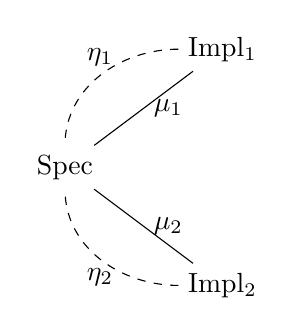
\begin{tikzpicture}
\node (S) at (0,0)
    {Spec};
\node (L1) at (2,1.5)
    {Impl$_1$};
\node (L2) at (2,-1.5)
    {Impl$_2$};
\draw[-\arrowtip](S) -- node[below,near end] {$\mu_1$} (L1);
\draw[-\arrowtip](S) -- node[above,near end] {$\mu_2$} (L2);
\draw[-\arrowtip,dashed](L1) to[out=180,in=90] node[above] {$\eta_1$} (S);
\draw[-\arrowtip,dashed](L2) to[out=180,in=-90] node[below] {$\eta_2$} (S);
\end{tikzpicture}
\end{center}

Challenge:
\begin{itemize}
\item collect initial library of mathematical concepts
\item collect alignments with individual libraries
% \lec{pairs of MMT identifiers}
\end{itemize}
\end{frame}


\section{OpenDreamKit}

\begin{frame}\frametitle{Virtual Research Environments for Mathematics}
\begin{itemize}
\item OpenDreamKit project 2015-2019  \hfill \emph{open PhD positions!}
\lec{EU project, 15 sites, 25 partners}
\lec{\url{http://opendreamkit.org/}}
\item Support full life-cycle
\begin{itemize}
\item exploration, development, and publication
\item archival and sharing of data and computation
\item real mathematicians as target audience
\end{itemize}
\item Key requirements
 \begin{itemize}
   \item allow using any foundation
     \lec{any programming language, database}
   \item integrate narration, computation, databases
   \item uniform user interfaces
 \end{itemize}
\end{itemize}
\end{frame}

\begin{frame}\frametitle{Math in the Middle Approach}
\begin{itemize}
\item Official definitions represented narratively
 \lec{MMT embedded into LaTeX to attach types}
\item Foundations written as MMT formal theories
\item Computation: library interfaces exported as MMT theories
\item Database schemata: written as formal MMT theories
\end{itemize}

Example work flow:
\begin{enumerate}
 \item user input mentions specific object
   \lec{e.g., the $13$th transitive group with conductor $5$}
 \item Systems $X$ queries MMT for $13a5$
 \item MMT retrieves object from connected databases
   \lec{e.g., LMFDb (L-functions and modular forms)}
 \item Database schema defines type and encoding of object
 \item MMT builds $13a5$ in high-level foundation
 \item MMT exports $13a5$ in input syntax of system $X$
\end{enumerate}
\end{frame}

\section{MMT-Based Foundation-Independent Results}

\begin{frame}\frametitle{Logical Result: Representation Language}
\begin{itemize}
 \item MMT theories uniformly represent
  \begin{itemize}
    \item logics, set theories, type theories, algebraic theories, ontologies, \ldots
    \item module system: state every result in smallest possible theory
     \lec{Bourbaki style applied to logic}
   \end{itemize}
  \item MMT theory morphisms uniformly represent
	   \begin{itemize}
	     \item extension and inheritance
	     \item semantics and models
	     \item logic translations
	    \end{itemize}
\item MMT objects uniformly represent
    \begin{itemize}
      \item functions/predicates, axioms/theorems, inference rules, \ldots
      \item expressions, types, formulas, proofs, \ldots
     \end{itemize}
\item \alert{Reuse principle}: theorems preserved along morphisms
\end{itemize}
\end{frame}

\begin{frame}\frametitle{Logical Result: Concepts}
MMT allows coherent formal definitions of essential concepts
\begin{itemize}
  \item Logics are MMT theories
  \item Foundations are MMT theories
  \lec{e.g., ZFC set theory}
  \item Semantics is an MMT theory morphism
  \lec{e.g., from FOL to ZFC}
%  For example,
%  \begin{itemize}
%    \item a logic $L$ is an MMT theory with a type of propositions
%    \item $L$-theories $T$ are extensions of $L$
%    \item a foundation is an MMT theory $F$ for, e.g., set theory
%    \item a semantics $S$ is an MMT morphism $L\to F$
%    \item $T$-models are MMT morphisms $S(T)\to F$
%  \end{itemize}
    \item Logic translations are MMT theory morphisms
    \item Logic combinations are MMT colimits
\end{itemize}
\end{frame}

\begin{frame}\frametitle{Logical Results: Algorithms}
	\begin{itemize}
		\item Module system \\
		  \lec{modularity transparent to foundation developer}
		\item Concrete/abstract syntax \\
		  \lec{notation-based parsing/presentation}
		\item Interpreted symbols, literals \\
		  \lec{external model/implementation reflected into \mmt}
		\item Type reconstruction \\
		  \lec{foundation plugin supplies only core rules}
		\item Simplification \\
		  \lec{rule-based, integrated with type reconstruction}
		  \bigskip
		\item Theorem proving?
		\item Code generation? Computation?
	\end{itemize}
\end{frame}


\begin{frame}\frametitle{Modular Framework Definitions in MMT}
Individual features given by set of symbols, notations, rules
	\begin{itemize}
		\item $\lambda\Pi$
		\item Rewriting
		\item Polymorphism
		\item Subtyping (ongoing)
		\item \ldots
	\end{itemize}
\vspace{1cm}

Language definitions are modular themselves
\lec{e.g., Dedukti = LF + rewriting}
\end{frame}

%\begin{frame}\frametitle{Application-Independence}
%\begin{itemize}
%  \item Practical logic-related systems often application-\alert{specific}
%    \begin{itemize}
%      \item fixed functionality for fixed foundation
%        \lec{often: read-eval-print design}
%      \item many applications shallow, decay quickly
%    \end{itemize}
% \item MMT approach: application-\alert{independence}
%	\begin{enumerate}
%	  \item focus on API for MMT language
%	    \lec{data structures and high-level interfaces}
%	  \item encapsulate advanced functionality in reusable services
%	    \lec{e.g., theorem proving, search, \ldots}
%	  \item allow plugin interfaces for customization
%	    \lec{foundation-specific rules, parsers, change listeners, \ldots }
%	  \item build lightweight applications on top
%	    \lec{IDE, library manager, \ldots}
%	\end{enumerate}
%\end{itemize}
%\end{frame}


\begin{frame}\frametitle{Knowledge Management Results}
	\begin{itemize}
		\item Change management
		  \lec{recheck only if affected}
		\item Project management
		  \lec{indexing, building}
		\item Extensible export infrastructure
		  \lec{Scala, SVG graphs, LaTeX, HTML, \ldots}
		\item Search, querying
		  \lec{substitution-tree and relational index}
		\item Browser
		  \lec{interactive web browser}
		\item Editing
		  \lec{IDE-like graphical interface}
	\end{itemize}
\end{frame}

\begin{frame}\frametitle{IDE}
 \begin{itemize}
   \item Inspired by programming language IDEs
   \item Components
     \begin{itemize}
       \item jEdit text editor (in Java): graphical interface
       \item MMT API (in Scala)
       \item jEdit plugin to tie them together
        \lec{only $\sim 1000$ lines of glue code}
     \end{itemize}
%   \item Generic default implementations for
%      \begin{itemize}
%        \item parsing
%        \item type checking
%        \item simplification
%      \end{itemize}
%      \lec{all extensible through rules of plugins}
   \item Features
     \begin{itemize}
       \item outline view
       \item error list
       \item display of inferred information
       \item type inference of subterms
       \item hyperlinks: jump to definition
       \item search interface
       \item context-sensitive auto-completion: show identifiers that
%        \begin{itemize}
%          \item are in scope
%          \item have the right type
%        \end{itemize}
     \end{itemize}
\end{itemize}
\end{frame}

\begin{frame}\frametitle{IDE: Example View}
\includegraphics[width=\textwidth]{jedit-sidebar-errors.jpg}
\end{frame}

\begin{frame}\frametitle{An Interactive Library Browser}
\begin{itemize}
\item MMT content presented as HTML5+MathML pages
%\\[.5cm]
%\includegraphics[width=\textwidth]{web-proof-tree.jpg}
%\\[.5cm]
\item Dynamic page updates via Ajax
\item MMT used through HTTP interface with JavaScript wrapper
\item Features
  \begin{itemize}
    \item interactive display
      \lec{e.g., inferred types, redundant brackets}
    \item smart navigation via MMT ontology
       \lec{can be synchronized with jEdit}
    \item dynamic computation of content
       \lec{e.g., definition lookup, type inference}
    \item graph view: theory diagram as SVG
  \end{itemize}
\end{itemize}
\end{frame}


\begin{frame}\frametitle{Browser: Example View}
\includegraphics[width=\textwidth]{browse.jpg}
\end{frame}

\begin{frame}\frametitle{Browser Features: 2-dimensional Notations}
\includegraphics[width=\textwidth]{2dnot.jpg}
\end{frame}

\begin{frame}\frametitle{Browser Features: Proof Trees}
\includegraphics[width=\textwidth]{web-big.jpg}
\end{frame}

\begin{frame}\frametitle{Browser Features: Type Inferece}
\includegraphics[width=\textwidth]{type-inference.jpg}
\end{frame}

\begin{frame}\frametitle{Browser Features: Parsing}
\includegraphics[width=\textwidth]{parse.jpg}
\end{frame}

\begin{frame}\frametitle{Example Service: Search}
\includegraphics[width=\textwidth]{search.jpg}
\end{frame}

%\begin{frame}\frametitle{Pros and Cons}
%\begin{itemize}
%\item Advantages
% \begin{itemize}
%   \item generic logical results
%	 \item generic knowledge management
%	 \item high investment - high yield
%	   \lec{lots of applications become easy}
%	 \item long-term maintainability
%	   \lec{robustness under change of plan}
% \end{itemize}
%\item Disadvantages
%  \begin{itemize}
%    \item genericity can be hard to achieve
%    \item specialization to particular foundation+application needed
%  \end{itemize}
%\item MMT research hypothesis: foundation-/application-independence pays off
%  \lec{confirmed so far}
%\end{itemize}
%\end{frame}

\begin{frame}\frametitle{Envisioned: A Generic Theorem Prover}
\begin{itemize}
\item Theorem proving currently highly logic-specific
\item But many successful designs actually logic-independent, e.g.,
  \begin{itemize}
   \item Declarative proof languages
   \item Tactic languages
   \item Integration of decision procedures
   \item Axiom selection
   \item Modularity
  \end{itemize}
\end{itemize}

\begin{blockitems}{Claim}
\item Logic-specific implementations a historical accident
\item Possible to build MMT level proving technology
\end{blockitems}
\end{frame}

\begin{frame}\frametitle{Envisioned: Computational Knowledge}
\begin{itemize}
 \item So far: MMT focuses on declarative formal languages
 \item Goal: extend to programming languages
  \begin{itemize}
    \item understand key concepts foundation-independently
      \lec{state/effects, recursion, inheritance, \ldots}
    \item represent features modularly
    \item freely mix logic and computation
     \lec{share declarative aspects}
  \end{itemize}
 \item Syntax is (kind of) easy:
  \begin{itemize}
   \item programming languages are MMT theories
   \item classes/modules are MMT theories
   \item programs are expressions 
  \end{itemize}
 \item Semantics is open question: What is the general judgment?
\end{itemize}
%\begin{itemize}
%\item MMT language design
% \begin{itemize}
%    \item programming languages are foundations
%      \lec{represented as theories}
%    \item classes are theories
%      \lec{(with state)}
%    \item implementations are models
%     \lec{represented as theory morphism from spec. to prog. language}
%  \end{itemize}
%\item MMT system components
%  \begin{itemize}
%    \item programs = proofs
%    \item compiler+IDE = proof assistant
%    \item compile program = run proof script
%    \item run program = check proof
%    \item program synthesis = theorem proving
%  \end{itemize}
%     \lec{MMT to organize knowledge/communication across components}
%\item logic::induction as computation::coinduction?
%\end{itemize}
\end{frame}


%\begin{frame}\frametitle{Representing Verbal Knowledge}
% \item<2> Goal: extend to informal/natural language
%	   \begin{itemize}
%	    \item practical specifications rarely fully formal
%	    \item partial formalization: formalize only important parts
%	      \lec{less expensive, more realistic}
%	    \item partial validation via MMT
%	      \lec{graceful degradation to informal knowledge}
%      \item state: current PhD student at Jacobs University
%	      %\lec{state of the art for specifications in practice}
%	\end{itemize}
%\end{itemize}
%\end{frame}

%\begin{frame}\frametitle{System Integration}
%Long-term research agenda
%   \begin{itemize}
%     \item Past: LATIN, integration of logics
%     \item Present: OAF, integration of libraries
%     \item Future: UniFormal, integration of tools
%   \end{itemize}
%\bigskip
%
%MMT as central
%\begin{itemize}
%	\item representation language
%	\item knowledge manager
%	\item mediator between tools
%\end{itemize}
%of a universal integration framework
%\end{frame}

\section{Big Challenges}

\begin{frame}\frametitle{Exporting System Libraries}
Major interoperability obstacle
\begin{itemize}
\item Communities very focused on 
	\begin{itemize}
	\item honing their system
	\item curating their library
\end{itemize}
\item Little effort for making libraries accessible
\item Slowly improving
 \begin{itemize}
 \item more people interested in sharing and generic tools
 \item OAF a driving force
 \end{itemize}
\end{itemize}
MMT good candidate for truly universal standard
\end{frame}

\begin{frame}\frametitle{Universal Library of Elementary Knowledge}
Requirements
\begin{itemize}
\item language-independent
\item system-independent
\item easy to write for practitioners
\end{itemize}

Vision
\begin{itemize}
\item Central library uses modular library of language features
\item Focus on names, types, properties
 \lec{no definitions, no proofs}
\item Individual contributions piece together minimal needed language
\item All existing systems
  \begin{itemize}
   \item remain in use
     \lec{e.g., for optimized proof support}
   \item allow refactoring results for submission to central library
  \end{itemize} 
\end{itemize}
\end{frame}


%\begin{frame}\frametitle{Universal System Integration: MMT as Mediator}
%\begin{itemize}
% \item Typical:
%   \begin{itemize}
%     \item isolated paradigm-\alert{specific} applications
%     \item with overlapping knowledge bases
%       \begin{itemize}
%         \item informal -- word processor -- specification
%         \item programming -- compiler -- implementation
%         \item logical -- theorem prover -- formalization
%       \end{itemize}
%   \end{itemize}
% \item MMT approach: paradigm-\alert{independence}
%   \begin{itemize}
%     \item MMT maintains shared knowledge space across tools
%     \item tools register reusable knowledge fragments with MMT
%       \lec{export as MMT theories}
%		  \begin{itemize}
%		    \item informal language: partial formalization
%		    \item programming language: function headers but not bodies
%		    \item logic: theorems but not proofs
%		  \end{itemize}
%	 \end{itemize}
% \item Goal: semantics-aware tool integration \\
%       while maintaining existing work flows
%\end{itemize}
%\end{frame}
%
%\begin{frame}\frametitle{Universal System Integration: MMT as Interface Generator}
%\begin{itemize}
% \item Similar to parser/interface generation frameworks
%   \lec{e.g., UML, Protocol Buffers}
% \item But generalized to logic/type theory
% \item Formalize theory diagram in MMT
%   \begin{itemize}
%     \item declarative
%     \item foundation-independent
%   \end{itemize}
% \item Export theory diagram to peripheral tools
%     \lec{part of MMT build tool}
%   \begin{itemize}
%     \item foundation-specific tools
%     \item {\LaTeX} packages
%     \item class diagrams, (de)serialization code
%     \item testing code \lec{generated from axioms}
%     \item documentation website
%   \end{itemize}
% \item Goal: synchronize knowledge bases through central definition
%\end{itemize}
%\end{frame}
%
%\begin{frame}\frametitle{Interface Generation: Example}
%\begin{itemize}
% \item LMFDB
%   \begin{itemize}
%     \item collaboration of $\sim 40$ mathematicians in number theory
%     \item goal: integrate multiple related but isolated knowledge bases
%   \end{itemize}
% \item Problems
%  \begin{itemize}
%    \item semantic relations often unclear
%    \item incompatible encodings for knowledge exchange
%  \end{itemize}
% \item Planned use of MMT:
%    \begin{enumerate}
%     \item mathematicians define central theories in MMT
%       \lec{close to mathematical language due to foundation-independence}
%     \item MMT generates
%       \begin{itemize}
%         \item interface classes
%         \item testing functions
%         \item database schemata
%         \item encoding/decoding functions
%         \item documentation websites
%       \end{itemize}
%   \end{enumerate}
%\end{itemize}
%\end{frame}

\begin{frame}\frametitle{Summary}
\begin{itemize}
\item MMT: foundation-independent framework for declarative languages
  \begin{itemize}
     \item representation language
     \item implementation
  \end{itemize}
\item Easy to instantiate with specific foundations
   \lec{rapid prototyping logic systems}
\item Deep foundation-independent results
   \begin{itemize}
   \item logical: parsing, type reconstruction, module system, \ldots
   \item knowledge management: search, browser, IDE, \ldots
   \end{itemize}
\item MMT quite mature now, ready for larger applications \lec{about to break even}
\item Serious contender for
 \begin{itemize}
  \item universal library
  \item generic applications/services
  \item system integration/combination
 \end{itemize}
% \begin{itemize}
%  \item new, changing foundations
%  \item generic applications/services
%  \item system integration/combination
% \end{itemize}
\end{itemize}
\end{frame}

\section{}


\newcommand{\link}[1]{} %\glec{\footnotesize\url{https://kwarc.info/people/frabe/Research/#1}}}
\newcommand{\papertitle}[1]{\footnotesize\textit{#1}}
\begin{frame}\frametitle{Further Resources}
\footnotesize
Web sites
\begin{itemize}
 \item MMT: \glec{\url{http://uniformal.github.io}}
 \item OAF web server (experimental): \glec{\url{http://mathhub.info:8080/}}
\end{itemize}
Selected publications
 \glec{all available from \url{https://kwarc.info/people/frabe}}
\begin{itemize}
    \item the primary paper on the MMT language (I\&C 2013, with M. Kohlhase):\\
      \papertitle{A Scalable Module System}
     \link{RK_mmt_10.pdf}
    \item a more recent paper on the MMT approach to logic (JLC 2014):\\
     \papertitle{How to Identify, Translate, and Combine Logics?}
    \link{rabe_howto_14.pdf}
    \item Foundations in LATIN: (MSCS 2011, with M. Iancu) \\
       \papertitle{Formalizing Foundations of Mathematics}
       \link{IR_foundations_10.pdf}
    \item Modular logics in LATIN (TCS 2011, with F. Horozal):\\
      \papertitle{Representing Model Theory in a Type-Theoretical Logical Framework}
      \link{HR_folsound_10.pdf}
    \item the primary paper on OAF (under review 2015, with M. Kohlhase) \\
       \papertitle{QED Reloaded}
       \link{KR_qed_14.pdf}
    \item Mizar in OAF (JAR 2013, with M. Iancu, M. Kohlhase, J. Urban):\\
      \papertitle{The Mizar Mathematical Library in OMDoc: Translation and Applications}
      \link{IKRU_mizar_11.pdf}
    \item HOL Light in OAF: (CICM 2014, with C. Kaliszyk)\\
       \papertitle{Towards Knowledge Management for HOL Light}     
       \link{KR_hollight_14.pdf}
\end{itemize}
\end{frame}

% % % % % % % % % % % % % % % % % % % % % % % % % % % % % % %
\section{Details: Foundations}
\input{foundations}
% % % % % % % % % % % % % % % % % % % % % % % % % % % % % % %

% % % % % % % % % % % % % % % % % % % % % % % % % % % % % % %
\section{Details: Logical Frameworks}
\input{logical_frameworks}
% % % % % % % % % % % % % % % % % % % % % % % % % % % % % % %

% % % % % % % % % % % % % % % % % % % % % % % % % % % % % % %
\section{Details: MMT Syntax}
\input{syntax}
% % % % % % % % % % % % % % % % % % % % % % % % % % % % % % %

% % % % % % % % % % % % % % % % % % % % % % % % % % % % % % %
\section{Details: Typing}
\input{typing}
% % % % % % % % % % % % % % % % % % % % % % % % % % % % % % %

% % % % % % % % % % % % % % % % % % % % % % % % % % % % % % %
\section{Details: Theory Morphisms}
\input{morphisms}
% % % % % % % % % % % % % % % % % % % % % % % % % % % % % % %

% % % % % % % % % % % % % % % % % % % % % % % % % % % % % % %
\section{Details: LATIN}
\input{latin}
% % % % % % % % % % % % % % % % % % % % % % % % % % % % % % %

% % % % % % % % % % % % % % % % % % % % % % % % % % % % % % %
\section{Details: Open Archive of Formalizations}
\input{oaf}
% % % % % % % % % % % % % % % % % % % % % % % % % % % % % % %

% % % % % % % % % % % % % % % % % % % % % % % % % % % % % % %
\section{Details: Systems}
\input{systems}
% % % % % % % % % % % % % % % % % % % % % % % % % % % % % % %

\end{document}


% frame templates
\begin{frame}\frametitle
\begin{center}
\end{center}
\end{frame}

\begin{frame}\frametitle{}
\begin{itemize}
\item 
\item 
\item 
\item 
\end{itemize}
\end{frame}

\begin{frame}[fragile]\frametitle{}
\begin{lstlisting}
\end{lstlisting}

\end{frame}

\framebox{
\begin{tikzpicture}
\node[circle,draw] (A) at (1,0)
    {$A$};
\node (B) at (5,0)
    {$B$};
\node (C) at (9,0)
    {$C$};
\node (c) at (5,2) {$c$};
\node (i) at (-1,1) {$i$};
\draw[-triangle 45](A) -- node[above] {$f$} (B);
\draw[-](B) -- node[above] {$a$} (C);
\draw[->](A) .. controls (c) .. (C);
\draw[<-](A) .. controls (i) and (-1,-1) .. (A);
\end{tikzpicture}
}

\begin{center}
\framebox{
\begin{minipage}{\textwidth}

\end{minipage}
}
\end{center}

\begin{tabular}{ll}
   \framebox{
     \begin{minipage}{0.45\textwidth}

     \end{minipage}
   }
  \end{minipage}
&
  \framebox{
    \begin{minipage}{0.45\textwidth}
    
    \end{minipage}
  }
\\
\end{tabular}
\end{frame}
